%% FEUP THESIS STYLE for LaTeX2e
%% how to use feupteses (portuguese version)
%%
%% FEUP, JCL & JCF, 31 Jul 2012
%%
%% PLEASE send improvements to jlopes at fe.up.pt and to jcf at fe.up.pt
%%

%%========================================
%% Commands: pdflatex tese
%%           bibtex tese
%%           makeindex tese (only if creating an index) 
%%           pdflatex tese
%% Alternative:
%%          latexmk -pdf tese.tex
%%========================================

\documentclass[11pt,a4paper,twoside,openright]{report}

%% For iso-8859-1 (latin1), comment next line and uncomment the second line
\usepackage[utf8]{inputenc}
%\usepackage[latin1]{inputenc}

%% Portuguese version

%% MIEIC options
\usepackage[portugues,mieic]{feupteses}
%\usepackage[portugues,mieic,juri]{feupteses}
%\usepackage[portugues,mieic,final]{feupteses}
%\usepackage[portugues,mieic,final,onpaper]{feupteses}

%% Options: 
%% - portugues: titles, etc in portuguese
%% - onpaper: links are not shown (for paper versions)
%% - backrefs: include back references from bibliography to citation place

%% Uncomment the next lines if side by side graphics used
%\usepackage[lofdepth,lotdepth]{subfig}
%\usepackage{graphicx}
%\usepackage{float}

%% Include color package
\usepackage{color}
\definecolor{cloudwhite}{cmyk}{0,0,0,0.025}

%% Include source-code listings package
\usepackage{listings}
\lstset{ %
 language=C,                        % choose the language of the code
 basicstyle=\footnotesize\ttfamily,
 keywordstyle=\bfseries,
 numbers=left,                      % where to put the line-numbers
 numberstyle=\scriptsize\texttt,    % the size of the fonts that are used for the line-numbers
 stepnumber=1,                      % the step between two line-numbers. If it's 1 each line will be numbered
 numbersep=8pt,                     % how far the line-numbers are from the code
 frame=tb,
 float=htb,
 aboveskip=8mm,
 belowskip=4mm,
 backgroundcolor=\color{cloudwhite},
 showspaces=false,                  % show spaces adding particular underscores
 showstringspaces=false,            % underline spaces within strings
 showtabs=false,                    % show tabs within strings adding particular underscores
 tabsize=2,	                    % sets default tabsize to 2 spaces
 captionpos=b,                      % sets the caption-position to bottom
 breaklines=true,                   % sets automatic line breaking
 breakatwhitespace=false,           % sets if automatic breaks should only happen at whitespace
 escapeinside={\%*}{*)},            % if you want to add a comment within your code
 morekeywords={*,var,template,new}  % if you want to add more keywords to the set
}

%% Uncomment next line to set the depth of sectional units listed in the toc
%\setcounter{tocdepth}{3}

%% Uncomment to create an index (at the end of the document)
%\makeindex

%% Path to the figures directory
%% TIP: use folder ``figures'' to keep all your figures
\graphicspath{{figures/}}

%%----------------------------------------
%% TIP: if you want to define more macros, use an external file to keep them
%some macro definitions

% format
\newcommand{\class}[1]{{\normalfont\slshape #1\/}}

% entities
\newcommand{\Feup}{Faculdade de Engenharia da Universidade do Porto}

\newcommand{\svg}{\class{SVG}}
\newcommand{\scada}{\class{SCADA}}
\newcommand{\scadadms}{\class{SCADA/DMS}}

%%----------------------------------------

%%========================================
%% Start of document
%%========================================
\begin{document}

%%----------------------------------------
%% Information about the work
%%----------------------------------------
\title{Sistema de Processamento e Análise Semântica de Redes Sociais para as Cidades Inteligentes}
\author{João Filipe Figueiredo Pereira}

%% Uncomment next line for date of submission
%\thesisdate{31 de Julho de 2008}

%% Uncomment next line for copyright text if used
%\copyrightnotice{Nome do Autor, 2008}

\supervisor{Orientador}{Rosaldo José Fernandes Rossetti}
\supervisor{Coorientador}{Pedro dos Santos Saleiro da Cruz}

%% Uncomment next line if necessary
%\supervisor{Co-orientador}{Nome de Outro Orientador}

%% Uncomment committee stuff in the final version
%\committeetext{Aprovado em provas públicas pelo Júri:}
%\committeemember{Presidente}{Nome do presidente do júri}
%\committeemember{Arguente}{Nome do arguente do júri}
%\committeemember{Vogal}{Nome do vogal do júri}
%\signature

%% Specify cover logo (in folder ``figures'')
\logo{uporto-feup.pdf}

%% Uncomment next line for additional text below the author's name (front page)
%\additionalfronttext{Preparação da Dissertação}

%%----------------------------------------
%% Preliminary materials
%%----------------------------------------

% remove unnecessary \include{} commands
\begin{Prolog}
  \chapter*{Resumo}

O Resumo fornece ao leitor um sumário do conteúdo da dissertação.
Deverá ser breve mas conter detalhe suficiente e, uma vez que é a porta
de entrada para a dissertação, deverá dar ao leitor uma boa impressão
inicial.

Este texto inicial da dissertação é escrito no fim e resume numa
página, sem referências externas, o tema e o contexto do trabalho, a
motivação e os objectivos, as metodologias e técnicas empregues, os
principais resultados alcançados e as conclusões.

Este documento ilustra o formato a usar em dissertações na \Feup.
São dados exemplos de margens, cabeçalhos, títulos, paginação, estilos
de índices, etc. 
São ainda dados exemplos de formatação de citações, figuras e tabelas,
equações, referências cruzadas, lista de referências e índices.
%Este documento não pretende exemplificar conteúdos a usar. 
É usado texto descartável, \emph{Loren Ipsum}, para preencher a
dissertação por forma a ilustrar os formatos.

Seguem-se umas notas breves mas muito importantes sobre a versão 
provisória e a versão final do documento. 
A versão provisória, depois de verificada pelo orientador e de 
corrigida em contexto pelo autor, deve ser publicada na página 
pessoal de cada estudante/dissertação, juntamente com os dois 
resumos, em português e em inglês; deve manter a marca da água, 
assim como a numeração de linhas conforme aqui se demonstra.

A versão definitiva, a produzir somente após a defesa, em versão 
impressa (dois exemplares com capas próprias FEUP) e em versão 
eletrónica (6 CDs com "rodela" própria FEUP), deve ser limpa da marca de 
água e da numeração de linhas e deve conter a identificação, na primeira 
página, dos elementos do júri respetivo. 
Deve ainda, se for o caso, ser corrigida de acordo com as instruções 
recebidas dos elementos júri.

Lorem ipsum dolor sit amet, consectetuer adipiscing elit. Sed vehicula
lorem commodo dui. Fusce mollis feugiat elit. Cum sociis natoque
penatibus et magnis dis parturient montes, nascetur ridiculus
mus. Donec eu quam. Aenean consectetuer odio quis nisi. Fusce molestie
metus sed neque. Praesent nulla. Donec quis urna. Pellentesque
hendrerit vulputate nunc. Donec id eros et leo ullamcorper
placerat. Curabitur aliquam tellus et diam. 

Ut tortor. Morbi eget elit. Maecenas nec risus. Sed ultricies. Sed
scelerisque libero faucibus sem. Nullam molestie leo quis
tellus. Donec ipsum. Nulla lobortis purus pharetra turpis. Nulla
laoreet, arcu nec hendrerit vulputate, tortor elit eleifend turpis, et
aliquam leo metus in dolor. Praesent sed nulla. Mauris ac augue. Cras
ac orci. Etiam sed urna eget nulla sodales venenatis. Donec faucibus
ante eget dui. Nam magna. Suspendisse sollicitudin est et mi. 

Phasellus ullamcorper justo id risus. Nunc in leo. Mauris auctor
lectus vitae est lacinia egestas. Nulla faucibus erat sit amet lectus
varius semper. Praesent ultrices vehicula orci. Nam at metus. Aenean
eget lorem nec purus feugiat molestie. Phasellus fringilla nulla ac
risus. Aliquam elementum aliquam velit. Aenean nunc odio, lobortis id,
dictum et, rutrum ac, ipsum. 

Ut tortor. Morbi eget elit. Maecenas nec risus. Sed ultricies. Sed
scelerisque libero faucibus sem. Nullam molestie leo quis
tellus. Donec ipsum. 

\chapter*{Abstract}

Here goes the abstract written in English.

Lorem ipsum dolor sit amet, consectetuer adipiscing elit. Sed vehicula
lorem commodo dui. Fusce mollis feugiat elit. Cum sociis natoque
penatibus et magnis dis parturient montes, nascetur ridiculus
mus. Donec eu quam. Aenean consectetuer odio quis nisi. Fusce molestie
metus sed neque. Praesent nulla. Donec quis urna. Pellentesque
hendrerit vulputate nunc. Donec id eros et leo ullamcorper
placerat. Curabitur aliquam tellus et diam. 

Ut tortor. Morbi eget elit. Maecenas nec risus. Sed ultricies. Sed
scelerisque libero faucibus sem. Nullam molestie leo quis
tellus. Donec ipsum. Nulla lobortis purus pharetra turpis. Nulla
laoreet, arcu nec hendrerit vulputate, tortor elit eleifend turpis, et
aliquam leo metus in dolor. Praesent sed nulla. Mauris ac augue. Cras
ac orci. Etiam sed urna eget nulla sodales venenatis. Donec faucibus
ante eget dui. Nam magna. Suspendisse sollicitudin est et mi. 

Fusce sed ipsum vel velit imperdiet dictum. Sed nisi purus, dapibus
ut, iaculis ac, placerat id, purus. Integer aliquet elementum
libero. Phasellus facilisis leo eget elit. Nullam nisi magna, ornare
at, aliquet et, porta id, odio. Sed volutpat tellus consectetuer
ligula. Phasellus turpis augue, malesuada et, placerat fringilla,
ornare nec, eros. Class aptent taciti sociosqu ad litora torquent per
conubia nostra, per inceptos himenaeos. Vivamus ornare quam nec sem
mattis vulputate. Nullam porta, diam nec porta mollis, orci leo
condimentum sapien, quis venenatis mi dolor a metus. Nullam
mollis. Aenean metus massa, pellentesque sit amet, sagittis eget,
tincidunt in, arcu. Vestibulum porta laoreet tortor. Nullam mollis
elit nec justo. In nulla ligula, pellentesque sit amet, consequat sed,
faucibus id, velit. Fusce purus. Quisque sagittis urna at quam. Ut eu
lacus. Maecenas tortor nibh, ultricies nec, vestibulum varius, egestas
id, sapien. 

Phasellus ullamcorper justo id risus. Nunc in leo. Mauris auctor
lectus vitae est lacinia egestas. Nulla faucibus erat sit amet lectus
varius semper. Praesent ultrices vehicula orci. Nam at metus. Aenean
eget lorem nec purus feugiat molestie. Phasellus fringilla nulla ac
risus. Aliquam elementum aliquam velit. Aenean nunc odio, lobortis id,
dictum et, rutrum ac, ipsum. 

Ut tortor. Morbi eget elit. Maecenas nec risus. Sed ultricies. Sed
scelerisque libero faucibus sem. Nullam molestie leo quis
tellus. Donec ipsum. Nulla lobortis purus pharetra turpis. Nulla
laoreet, arcu nec hendrerit vulputate, tortor elit eleifend turpis, et
aliquam leo metus in dolor. Praesent sed nulla. Mauris ac augue. Cras
ac orci. Etiam sed urna eget nulla sodales venenatis. Donec faucibus
ante eget dui. Nam magna. Suspendisse sollicitudin est et mi. 

Phasellus ullamcorper justo id risus. Nunc in leo. Mauris auctor
lectus vitae est lacinia egestas. Nulla faucibus erat sit amet lectus
varius semper. Praesent ultrices vehicula orci. Nam at metus. Aenean
eget lorem nec purus feugiat molestie. Phasellus fringilla nulla ac
risus. Aliquam elementum aliquam velit. Aenean nunc odio, lobortis id,
dictum et, rutrum ac, ipsum. 

Ut tortor. Morbi eget elit. Maecenas nec risus. Sed ultricies. Sed
scelerisque libero faucibus sem. Nullam molestie leo quis
tellus. Donec ipsum. 
 % the abstract
  \chapter*{Acknowledgements}

First of all, my deep gratitude to my friends for being on my side when I was a bit down.

\medskip

To my companions at Lab I120, João Neto, José Pinto, João Pedro Dias and Luís Reis ($\rho$7 Boyz): thank you for the funny moments during the whole dissertation period, specifically, during the tough process of writing up the document.

\medskip

To my colleagues, specially, Henrique Ferrolho: thank you for the friendship, patience and support in these five long years. Now, I am sure that more challenges are coming to us which may imply distance but besides that I truly believe that in the future we still would cross paths at the professional or even academic course.

\medskip

To Professor Rosaldo Rossetti and Pedro Saleiro, thank you very much for all support, dedication, enthusiasm and knowledge passed to me. During each task you defined in the dissertation period, I was able to improve myself in both academic and social levels.

\medskip

To the institution that host me, Faculty of Engineering of University of Porto (FEUP), as well as to all of its docents that guide me during this Master's program, I am thankful for everything I have learn until now.

\medskip

Last and more important, I would like to express my deep gratitude to my mother, Ana Brito, and my father, Júlio Pereira, for all the sacrifice and effort made to assure my future and concede me this opportunity to fulfil a dream: be graduated. I hope this achievement of mine make you very proud and I wish all success for both mine and your's ambitions and goals in the future. Like always, you know that you can count on me for everything you need.

\vspace{10mm}
\flushright{João Pereira}
  % the acknowledgments
  \cleardoublepage
\thispagestyle{plain}

\vspace*{8cm}

\begin{flushright}
   \textsl{``You should be glad that bridge fell down. \\
           I was planning to build thirteen more to that same design''} \\
\vspace*{1.5cm}
           Isambard Kingdom Brunel
\end{flushright}
    % initial quotation if desired
  \cleardoublepage
  \pdfbookmark[0]{Conteúdo}{contents}
  \tableofcontents
  \cleardoublepage
  \pdfbookmark[0]{Lista de Figuras}{figures}
  \listoffigures
  \cleardoublepage
  \pdfbookmark[0]{Lista de Tabelas}{tables}
  \listoftables
  \chapter*{Abreviaturas e Símbolos}
%\addcontentsline{toc}{chapter}{Abbreviations}
\chaptermark{ABREVIATURAS E SÍMBOLOS}

\begin{flushleft}
\begin{tabular}{l p{0.8\linewidth}}
ADT      & Abstract Data Type\\
ANDF     & Architecture-Neutral Distribution Format\\
API      & Application Programming Interface\\
CAD      & Computer-Aided Design\\
CASE     & Computer-Aided Software Engineering\\
CORBA    & Common Object Request Broker Architecture\\
UNCOL    & UNiversal COmpiler-oriented Language\\
Loren    & Lorem ipsum dolor sit amet, consectetuer adipiscing
elit. Sed vehicula lorem commodo dui\\
WWW      & \emph{World Wide Web}
\end{tabular}
\end{flushleft}

  % the list of abbreviations used
\end{Prolog}

%%----------------------------------------
%% Body
%%----------------------------------------

\StartBody

%% TIP: use a separate file for each chapter
\chapter{Introduction} \label{chap:intro}

\minitoc \mtcskip \noindent

\section{Context and Motivation}\label{sec:context_motivation}

In the last few years, the rise of Web 2.0, seen as the evolution of conventional Web services into collaborative and social platforms~\cite{chi2008social}, conducted to an excessive amount of User Generated Content~\cite{kaplan2010users} (UGC) being placed \textit{online} by the population. Due to this emergency of web-content, the research community has been exploring it in order to extract added-value information regarding a large diversity of domains, such as opinion mining, human behavior and respective activity patterns, political issues, social communication (e.g. news websites). Social media platforms, more specifically, social media content (SMC), a type of UGC, has been targeted by several scientific researches focused mostly in the text mining area. Although the application of SMC in the previous mentioned domains, the \textit{smart cities}~\cite{batty2012smart} and, in particular, the transportation~\cite{gal2014potential} domain are under a smooth growth, meaning that a large path is still unexplored allowing new opportunities and challenges for the research community to reach its full potential~\cite{kn:Musto2015}.

Availability and authenticity are some of the social media content advantages considering that such information do not require additional costs regarding its exploration, is, \textit{a priori}, generated by humans, transcending a certain level of credibility and, lastly, due to the availability of tools provided by social media platforms, we can store the data and perform off-line analysis~\cite{kuflik2017automating}. Twitter is considered a MicroBlog, a type of social network, which content is similar to SMS-like messages, characteristic of a 140-characters length, and the 11th most visited website in the world~\footnote{http://www.alexa.com/siteinfo/twitter.com}. This platform has already proved its value and potential in domains ranging from news detection~\cite{kn:Sankaranarayanan2009} to real-time traffic sensing~\cite{carvalho2010real} being for this reason one of the most explored sources of data during the conduction of research studies.

Mining Twitter data is although the availability and free cost, a laborious and time-consuming process due to the restrictions and difficulties present in its content. The informal language, the existence of slang, abbreviations, jargons and the short length of the message are some of the problems when analyzing this data. Harvesting tweets automatically and, at the same time, extracting valuable information for the target domains delineated in this dissertation makes the task even more complex. However, by surpassing the previous mentioned problems, the extracted information may be of extremely importance and useful to the final stakeholders, namely \textit{smart cities} and transportation entities, during decision-making policies to improve their services.

\section{Problem Statement}\label{sec:problem}
The problem around this dissertation is focused in the analysis of a continuous flow of social media streams provided by Twitter. To analyse such streams, multiple steps composed in an iterative process are needed in order to filter out non-related content and proceed with extraction of information about a specific scenario. Here, since the target scenarios are associated to \textit{smart cities} and transportation domains, data related to it must be explored and analysed. To the best of our knowledge, there are no public datasets related to these domains and the creation of a gold standard dataset constitutes a complex endeavor, which is, for this reason, an obstacle to surpass in this dissertation. The extraction of information from social media content is another overwhelming task since it is necessary the application of several NLP methods in order to minimize/extinct its peculiarly problems. Hence, the main problem can be divided in five distinct sub-problems:

\begin{enumerate}
	\item \textbf{Data collection method for various locations}\\
	Choosing a method to collect data that provides a large range of valuable information for different cities constitutes the first sub-problem.
	
	\item \textbf{Content filtering}\\
	It is necessary the guarantee of that all information is fully related to the target scenario in the analysis, as well as removing messages which does not brought additional information (for instance, tweets only composed by \textit{emoticons}) or are not related to the end-users expectations, i.e. if we are targeting content from a specific city, we must assure that such content is indeed posted when users were there.
	
	\item \textbf{Identification of topics in Twitter messages}\\
	The identification of topics in Twitter messages is a very important point in the analyses of the \textit{smart cities} context. This task allows the identification of what is been talked about recently and also where the conversation topics are geographically distributed.
	
	\item \textbf{Travel-related classification}\\
	In order to produce valuable information for the transportation services, we need to analyse the content of a message and verify if it is truly related with the domain in study. Hence, discriminate travel-related tweets is one of the sub-problems that must be tackled.
	
	\item \textbf{Data aggregation and visualization}\\
	The aggregation of the results provide by all other tasks is needed. This aggregation task may be continuously calculating the results in order to make the user experience easier and smooth without taking to much response time by the data visualization UI. The graphical visualizations should be of easy interpretation by the end-user and having this in mind some qualitative and quantitative indicators may be presented.
\end{enumerate}

\section{Goals and Expected Contributions}\label{sec:contributions}
Following the previous mentioned problem in Section \ref{sec:problem}, the main goal of this dissertation passes through the development of a prototype framework based on the concept of analysis. Such framework demands a solution for each of the aforementioned sub-problems, and for that reason modularity is needed in the design and implementation of the final tool. Its usability will be directed to companies or even ordinary users and should be able to provide relevant information about a specific real-world scenario under the \textit{smart cities} and transportation fields. The framework should be capable of automatically processing social media texts, more specifically, general topic detection and characterization of travel-related tweets. The following list summarizes the crucial goals behind this dissertation:

\begin{itemize}
	\item Extraction of valuable information from Social Media Content to the Transportation and \textit{Smart Cities} domains;
	\item Designing and implementation of a framework capable of automatize the analysis process;
	\item Application, when possible, of recent advances in the area of text analysis;
\end{itemize}

\medskip

In terms of expected contributions, we hope that such generated information through the framework data analytics may be relevant both to ordinary users of a particular service and to the responsible entities in order to improve decision-making policies.

\section{Publications}\label{sec:publications}
In this section several scientific contributions performed during the period of this dissertation are mentioned:

\begin{itemize}
		\item
		João Pereira, Arian Pasquali, Pedro Saleiro and Rosaldo J. F. Rossetti. {\color{blue}Transportation in Social Media: an automatic classifier for travel-related tweets}. In \emph{Portuguese Conference on Artificial Intelligence} (EPIA), 2017. In Press.
		
		\item
		João Pereira, Arian Pasquali, Pedro Saleiro and Rosaldo J. F. Rossetti. {\color{blue}Classifying Travel-related Tweets using Word Embeddings}. In \emph{International Conference on Information and Knowledge Management} (CIKM), 2017. Under review.
		
		\item
		João Pereira, Arian Pasquali, Pedro Saleiro and Rosaldo J. F. Rossetti. {\color{blue}Characterizing Geo-located Tweets in Brazilian Megacities}. In \emph{IEEE International Summer School on Smart Cities} (IEEE S3C), 2017. Under review.
\end{itemize}

\section{Dissertation Structure}\label{sec:diss_structure}
The effort applied to this dissertation generated a great diversity of points and due to that the remainder of the document is structured into four chapters.
Section \ref{chap:sota} starts with a brief conceptualization in the Smart Cities and Intelligent Transportation System domains, as well as previous related works using social media content as its basis.
The proposed framework is referenced in Section \ref{chap:framework}, being each its composing modules depth described.
Experiments performed to test each module of the framework are reported in Section~\ref{chap:experiments}.
Completing this document, conclusions, future work and a few final remarks are exposed in chapter~\ref{chap:conclusions}. 
\chapter{Background and Literature Review} \label{chap:sota}

\minitoc \mtcskip \noindent

This section aims the analysis and reflection about some works that has as final goal, similarly to ours, the development of a framework with the purpose of exploring social media data to extract meaningful domain-specific information. Nonetheless, studying works from other authors may help or even find already proposed solutions in order to solve the aforementioned problems.

Hence, this section will contemplate a brief contextualization about how can an intelligent system contribute to the improvement of a \textit{smart city} or transportation services. Moreover, technologies and methods that allow extraction of information from a text document or, in this particular case, from tweets will be described. Finally, an exploration through already existent frameworks regarding the information extraction from social media content as well as the identification of its application domain.

\section{Smart Cities}\label{sec:smart_cities}

\textit{Smart City} is a concept appeared thanks to the continuous growth of a city's population which contributed to an aggressive level of urban and technological developments~\cite{kn:Cecilia2016}. In the last few years, several definitions for its meaning have emerged but its main idealization is not yet fully known~\cite{kn:Komninos2009}. Angelidou~\cite{kn:Angelidou2015} defined Smart City as

\emph{"Conceptual urban development model on the basis of the utilization of human, collective, and technological capital for the development of urban agglomerations"},

enhancing \textit{knowledge} and \textit{innovation economy} as the primary factors that support the development of a city. Alongside with the previous factors, the author identifies other three distinct forces that shape the concept of a \textit{smart city}:

\begin{enumerate}
	\item \textit{Technology Push}: The need of new products and solutions are introduced into the market due to a fast advance in science and technology.
	\item \textit{Demand Pull}: Current problems are solved originating new possibilities to respond society demands such as the continuous growth of the population.
	\item \textit{Urban Future}: Represents the final goal of a city constituting for that reason an important role in the whole transformation process.
	\item \textit{Knowledge and Innovation Economy}: The creation of new products using the most recent technologies is associated to solution for the efficiency and sustainability of a city.
\end{enumerate}

The first two forces previous mentioned are directly dependent of the other ones as it is showed in Figure~\ref{fig:four_forces}. However, the absence of desire to reach a better future having into consideration the city's economy and resources can result in the break of its dynamics and healthy, affecting services of a city due to the population discontentment.

\begin{figure}
	\centering
	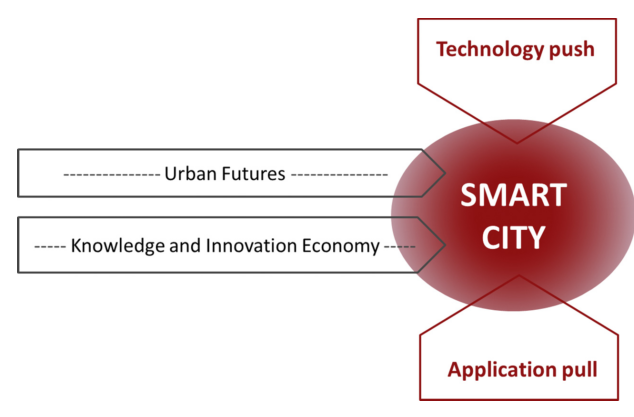
\includegraphics[width=0.6\textwidth]{figures/four_forces.png}
	\caption{\textit{Smart City} conjecture of four forces. Source:~\cite{kn:Angelidou2015}}
	\label{fig:four_forces}
\end{figure}

The development environment of a city tagged as \textit{smart} is another key factor to reach the success. Komninos~\cite{kn:Komninos2009} associates collective sources of innovation to the improvement of life quality in cities. The globalization of innovation networks is responsible for the emergency of another types of environments and infrastructures, as so \emph{"global innovation clusters and i-hubs, intelligent agglomerations, intelligent technology districts and intelligent clusters, living labs"} allowing the testing of products or services by the ordinary citizens in order to identify problems or even analyse their behaviour  and reactions regarding what have experimented~\cite{kn:Komninos2009}. Hence, it is possible to affirm that the development of a city has its starting point in the community but also depends on the quality of \glspl{ICT}~\cite{hollands2008will}, an essential requirement in the city's evolution process.

Last but not least, a \textit{smart city} may focus its efforts in several sectors, such as the environment, culture and recreation, education, social and economic aspects, demography, and travel and transportation~\cite{caragliu2011smart} in order to have equally advances in all of them.

\section{Intelligent Transportation Systems}\label{sec:intelligent_transportation_systems}

The transportation system is inherently connected to the progress of a city because people uses on a daily-basis transportation modes, i.e. bus, private cars, metropolitan, and others, in order to go to their jobs and make their own life and through that they contribute to the economic progress of it. Although this connection, such system is also influenced by the problem of population growth being relevant and necessary the finding of solutions to minimize or even erase it~\cite{kn:Caragliu2015}. Hence, "a \textit{smart city} should be focused on its actions to become smart", coming up the concept of innovation~\cite{kn:Cecilia2016}.

To understand what are \gls{ITS}, it is necessary to introduce the meaning of \gls{SM}. \gls{SM} is a combination of comprehensive and smarter traffic service with smart technology, enabling several intelligent traffic systems which provide control in the signals regarding the traffic volume, information about smooth traffic flows, times of bus, train, subway and flight arrivals, their routes or even the knowledge of what citizens thought about the city's services~\cite{kn:Chun2015}. The majority of \gls{ITS} are expressed through smart applications where transportation and traffic management has became more efficient and practicable, allowing the users to access important information about the transportation systems in order to make correct decisions about what they want to use in their cities~\cite{kn:Caragliu2015}. \gls{ICT}-based infrastructures are the main support for \textit{smart cities} and due to tha, they also serve as support to \gls{ITS}, since the information provide by such infrastructures allows the piloting of activities such as traffic operations, as well as its  management over a long period of time~\cite{kn:Cecilia2016}.

Nowadays, cities are exploring some initiatives of sensing to support the development of technological projects. Areas such as utilities management (where, for example, is monitored the consumption level of power, water and gas), traffic management (using vibration sensors to measure the traffic flows on bridges, or even the full capacity of a parking lot), environment awareness (using video cameras to monitor the population behaviour and sensors to measure the level of air pollution) make use of physical sensors, i.e. some devices that can capture information to study and improve the quality of life in a daily basis~\cite{kn:Doran2015}. Szabo et al.~\cite{kn:Szabo2013} and Doran et al.~\cite{kn:Doran2015} reported the highly economic cost to this kind of sensing, since it is require maintenance and replacement of this devices, as well as a tracking infrastructure to store and process the collected information. Hence, a new form of sensing has emerged - \gls{Crowdsensing} - offering to the cities several ways to improve their services by exploring the participation of the citizens through social networks where there is a publicly sharing of  opinions and thoughts regarding some problems around the city where they live are passing in~\cite{kn:Roitman2012}. This type of sensing consists in human-generated data provided by the population through the usage of mobile devices and social networks web-based platforms. Such data can be further used to extract some analytics regarding specific services in a city, namely the urban transportation system~\cite{kn:Roitman2012}. Having this considered, social media can be seen as a good source of data to extract valuable information aiming the direct use of it into the smartness evolution process of a city~\cite{kn:Szabo2013}. Recently, it is possible to verify that cities are increasingly opting for technological opportunities based on \textit{crowd sensing}, once this type of exploration brings a considerable reduction of costs and support in the development of news valuable technologies.

In the last few years, several authors have published a widely range of social-media-based contributions focusing this specific domain. Kurkcu et al.~\cite{kurkcu2016evaluating} use geo-located tweets to try and discover human mobility and activity patterns. The subject of transport modes was explored by Maghrebi et al.~\cite{maghrebi2016transportation} in the city of Melbourne, Australia. From a dataset of 300,000 geo-located tweets, authors tried to extract tweets related to several modes of transport using a keyword-based search method. 

Additionally, there were also different efforts focused on the tracking of accidents using Twitter social media data. Mai and Hranac~\cite{mai2013twitter} tried to establish a correlation between the California Highway Patrol incident reports and the increased volume of tweets posted at the time they were reported. On the other hand, Rebelo et al.~\cite{rebelo2015twitterjam} implemented a system capable of extract and analyse events related to road traffic, coined  TwitterJam. In that study, authors also used geo-located tweets that were already confirmed as being related to events on the roads and compared their counts with official sources.

Performing robustness experiments over this domain is challeging since although the large number of recently publications, gold standards are yet not defined or even public being for this reason difficult to prove the methodology chosen or suppositions made. Maghrebi et al.~\cite{maghrebi2016transportation} enhances some terms related to the transportation domain, however they are limited and also very common ones. After a tough investigation work, it is worth noting a list produced by Gal-Tzur et al.~\cite{gal2014potential} containing a large number of terms whose may serve as support for new  scientific contributions using social media in studies of the transportation domain.

\section{Social Media Analytics}

In the last few years social networks have made impact on the business communications since users assumed the role of costumers through the publication of content on these networks, rising high levels of interaction between them, as well as with businesses entities~\cite{kn:Cecilia2016}. A proof of that is the amount of information produced since 2011 which is equivalent to a number over than 90\% of the available data online~\cite{kn:SINTEF}. Facebook\footnote{\url{https://www.facebook.com/}}, Twitter\footnote{\url{https://twitter.com/}} and other social networking websites are nowadays used as business tools by companies aiming the efficient use of digital marketing techniques to publicize their products~\cite{kn:Royle2014}. Besides the business field, the population turn widely into this new communication technologies publicly sharing real-life events, their opinions about certain topics and their on-time feelings in the network through a simple message \cite{kn:DAndrea2015}.

Social Media Analytics (SMA) can be described as a type of digital analytics which focus is the study of interactions between, their opinions/thoughts, their own life, companies as so its products or services through the social media data. Such study provides important information to "analysts, brands, agencies or vendors" facilitating the generation of economic value to many organizations~\cite{kn:Judah2012}. In order to achieve the main goal of the SMA, companies focus their effort in the development automatic systems to make possible an easy collection, analysis, summarization and visualization of processed social media data establishing specific points about what is necessary to improved in their products~\cite{zeng2010social}.

However the potential value that SMA can provide, J. Phillips~\cite{kn:Judah2012} enhance some important factors to be considered in the analytics process: (1) Users permissions; (2) Awareness/listening of real-time information; (3) Search mechanisms; (4) Text analysis methodologies and techniques; (5) Data access and integration; (6) System integration, customization and growth.

The previous mentioned factors will help during the identification and comprehension of possible necessary features in a social media analytics tool, as well as to establish potential parameters/metrics to test and evaluate such tool. Without careful conduction in the social media tool elaboration, for instance, use of a wrong technique of SMA could have a bad business impact for the company resulting possible bankruptcies and increase the unemployment tax of a city.

%\subsection{Data Management}
%\subsection{The potential of Twitter}

\section{Text Mining}

Text mining is a conjecture of fields such as information retrieval, data mining, machine learning, statistics and computational linguistics which aims the extraction of valuable information from unstructured textual data~\cite{kn:He2013}. The intensively usage of this analysis methodology is due to the massive amount of information stored in text documents being necessary automatic techniques to identify, extract, manage and integrate the knowledge acquired from these texts exploration in a efficiently and systematically way~\cite{ananiadou2015textmining}. On the other hand, the emergency of social media applications have also contributed to the widely growth of text mining usage because of the "application’s perspective and the associated unique technical and social science challenges and opportunities"~\cite{zeng2010social}.

Text mining shares some of the issues presented by the Natural Language Processing (NLP) field. Texts are usually performed by humans and due to that, some problems in its construction can appear, such as spelling mistakes, wrong phrasal construction, slang among other. Before the mining process of a text, it's important to apply some preprocessing steps in order to eliminate or, at least reduce, undesired content (words) in the primary analysis process.
A. Stavrianou et al.~\cite{kn:Stavrianou2007} cite these issues very well alongside their work and some of them are observable in Table~\ref{table:textminingissues}.

\begin{table}[htbp]
	\centering
	\caption{Text Mining Issues by A. Stavrianou \cite{kn:Stavrianou2007}}
	\label{table:textminingissues}
	\begin{tabular}{ | l | p{7cm} |}
		\hline \textbf{Issue}            & \textbf{Details}\\
		\hline Stop list                 & Should we take into account stop words?\\ 
		\hline Stemming                  & Should we reduce the words to their stems?\\ 
		\hline Noisy Data                & Should the text be clear of noisy data?\\ 
		\hline Word Sense Disambiguation & Should we clarify the meaning of words in a text?\\ 
		\hline Part-of-speech Tagging    & What about data annotation and/or part of speech characteristics?\\ 
		\hline Collocations              & What about compound or technical terms?\\ 
		\hline Grammar / Syntax          & Should we make a syntatic or grammatical analysis? What about data dependency, anaphoric problems or scope ambiguity?\\ 
		\hline Tokenization              & Should we tokenize by words or phrases and if so, how?\\ 
		\hline Text Representation       & Which terms are important? Words or phrases? Nouns or adjectives? Which text model should we use? What about word order, context, and background knowledge? \\ 
		\hline Automated Learning        & Should we use categorization? Which similarity measures should be applied? \\ \hline
	\end{tabular}
\end{table}

The removal of words from text may sometimes not be desirable because some sentences can lose its information or even leads to a different meaning compared with its original form. The generation of a stop list words should be a supervised task as long as little words could induce distinct results in the text classification~\cite{kn:Riloff1995}.

Stemming is a task that depends mostly from the speaking language of the text than its specific domain~\cite{kn:Stavrianou2007}. The main goal of this technique is to reduce a word to its root form helping in the calculus of distances between texts, keywords or phrases, or even in the text representation.

The noisy data is derived from spelling mistakes, acronyms and abbreviations in texts and to solve this, a conversion of these terms should be done to maintain the integrity of data. Commonly solution approaches involve text edit distances (Levenshtein Distance\footnote{\url{https://en.wikipedia.org/wiki/Levenshtein_distance}}) and phonetic distances measures between known words and the misspelling ones to achieve good corrections~\cite{kn:Bontcheva2013} 

Word Sense Disambiguation (WSD) focus on solving the ambiguity in the meaning of a word. Other similar field to WSD is Name Entity Disambiguation (NED) where the disambiguation target are named-entities mentions, while WSD focus on common words. WordNet\footnote{\url{https://wordnet.princeton.edu/}} is a commonly used resource to extinguish this ambiguity \cite{kn:Chang2016}. There are two types of disambiguation: the unsupervised, where the task is support by a dictionary or a thesaurus \cite{kn:Stavrianou2007}; and, the supervised one, where different meanings of a word are unknown and normally learning algorithms with training examples are used to achieve good results regarding the performance of the disambiguation task~\cite{kn:Yarowsky1995}.

Tagging can be describe as the process of labeling each term of the text with a part-of-speech tag, i.e. classify each word as a noun, verb, adjective, and others \cite{kn:Hotho2005}. Collocations are groups and constitutes a very important step in some text mining approaches. Grouping two or more words to give its correct meaning is sometimes crucial to perform tasks such as sentiment analysis where negations (e.g. "don't like") needed to be composed by two or more words in order to assure the negative value of, for example, a verb. Collocations are usually made before the WSD task since some compound technical terms have different meaning from the individual words which composed it \cite{kn:Stavrianou2007}.

Tokenization serves to pick up all the terms presented in a text document and to achieve this it's necessary splitting its content into a stream of words implying the removal of the punctuation marks and non-text characters \cite{kn:Hotho2005}. Some authors also see tokenization as a text representation form since one of the most used models to represent texts is \textit{Bag-of-words} (BoW). This model broke down texts into words and stores it in a term-frequency vector according the occurrence of a word in the text. Hence, each word may represent a feature \cite{kn:Sriram2010}. Another commonly used model to represent texts is Vector Space Models that represent all the documents in a multi-dimensional space where documents are converted to vectors and each vector may be seen as a feature. This model provides some advantages since the documents can be compared with each other by performing some specific vector operations \cite{kn:Hotho2005}.

Once been introduced some of the most preliminary important steps in text mining, the remainder subsection are focused in two different text analytics approaches: text classification and topic modelling. The majority of Social Media Analytics approaches focus its efforts in modelling and classification in order to understand the large range of data collected and support commonly used techniques to extract information from it, such as sentiment analysis, trend analysis and topic modeling~\cite{kn:Fan2013}.

\subsection{Text Classification}

Text classification is a text mining task which main goal is the discrimination or characterization of a piece of text into a specific format value. Such value can vary from number (sentiment analysis tasks), labels (multi-labeling tasks), classes (binary or multi-class tasks). Classification in text analysis is a widely used methodology and had already been reported in several scientic contributions regarding the smart cities and transportation domains.

Support Vector Machines (SVM)~\cite{signorini2011use, zhang2016mining, pereira2017transportation, carvalho2010real}, Ordinary Least Squares (OLS)~\cite{saleiro2016sentiment}, Random Forests (RF)~\cite{saleiro2017feup}, MultiLayer Perceptron (MLP)~\cite{saleiro2017texrep}, Naïve Bayes (NB) and Decision Trees J48 (DT J48)~\cite{kuflik2017automating} are some of the supervised classification models used to analyse social media data over fields such as health and pharmacovigilance, political opinion, transportation (travel classification, traffic and incidents detection), financial sentiment analysis and \textit{online} reputation monitoring.

A. Sifnorini et al.~\cite{signorini2011use} reported a study which main goal was the tracking of the disease Influenza A (H1N1) virus. Tweets collected by the authors using term-based search sum up more than 300 million examples. Their methodology consists in training SVM models with sets of frequency features composed by the most used weekly-terms over the whole dataset. Each model was specifically trained according a certain set of keywords and follow an iterative process, i.e. authors firstly have classified all illness-related tweets related and than used the resulting related subset of data to perform new classification regarding specific keywords, such as what was the disease source, countermeasures used and infected people characteristics. Final results allowed the verification of a decrease of Twitter activity while more new cases were appearing meaning less concerning about this epidemic through time.

Accident-related classification for Twitter data was proposed by Z. Zhang et al.~\cite{zhang2016mining}. Authors explored the Twitter Streaming API to collect geo-located tweets from Northern Virginia during a completed year, January to December of 2014, and recurring to auxiliary loop detectors that are, in intervals of 15 minutes, recording the traffic flow. In order to automatize the detection of accidents in that interval of time (were the sensors are not recording the scene), authors have built a binary classification model using Linear SVM with a balanced dataset composed by 400 training examples for each of the accident-related and non-related classes composed by a boolean-vectors according the final 3,000 tokens resulted from the token filtering and stemming process. Performance was improved by submitting the model to a 5-fold cross validation which was proved by values of accuracy and precision over than 70\% of success.

%J. Pereira et al.~\cite{pereira2017transportation} try to discriminate travel-related tweets recurring to a combination of two different types of features: bag-of-words and word embeddings. Authors explored almost 9,000,000 geo-located tweets from two Brazilian \textit{megacities} and construct, manually, a balanced training dataset of travel-related and non-related tweets. The binary classification proved to have better performance under the SVM model experiments with linear \textit{kernel} function, as well as the two previous mentioned works here.

Considering the task of discriminate travel-related tweets, S. Carvalho et al.~\cite{carvalho2010real} have constructed a bag-of-words dependent classification model and achieved improvements at the model's performance with support of a bootstrapping approach implying a two phases train to the SVM model.  By assuming the similarities, i.e. all four works were related to binary text classifications, we can induce an hypotheses that Linear SVM models have superior performances relatively to other models for this type of classification tasks.

Multi-class classification models were also applied to the transportation domain through text analysis of social media content. T. Kufliket al~\cite{kuflik2017automating} build multiple classification models using methods such as Naïve Bayes and Decision Trees (J48) to predict multiple modes of transport during three different sports events. Tweets sum up a total of 3.7M and were submitted to the models classification task in order to prove that an harvesting automatically information from Social Media Content is possible and may help transportation entities in the planning and management of their services during social occasions as it is demonstrate in theirs use cases.

On the other hand, P. Saleiro et al.~\cite{saleiro2016sentiment} tried to predict the 2011 Portuguese bailout results analysing the tweets opinion about all five political parties candidates. The opinion was measure using a OLS model trained with specific sentiment aggregate functions and proved to be capable of correctly predict who would be elected prime minister of Portugal only exploring sentiment analysis in social media data. In SemEval-2017 Task 5, P. Saleiro et al. explored word embeddings techniques to extract the sentiment polarity and intensity in financial-related tweets. Authors have proved good performance of models trained with bag-of-words and bag-of-embeddings features together although the approach been applied to a specific domain. The usage of features representing syntactic and semantic similarities of texts, such as word embeddings, can be seen with great potential namely to the area of travel-related text classification.

\begin{table}[htbp]
	\centering
	\caption{Brief overview of the related work for text classification - Best Experiments}
	\label{my-label}
	\resizebox{\textwidth}{!}{\begin{tabular}{c|c|c|c|c}
			\hline
			\textbf{Approach} & \textbf{Features} & \textbf{Classification Methods} & \textbf{Goal} & \textbf{Potential Domain}\\ \hline
			A. Sifnorini et al.~\cite{signorini2011use} & Bag-of-words & Linear SVM & \begin{tabular}[c]{@{}c@{}}Tracking the evolution of public sentiment\\ and increasing of social media activity about\\ the H1N1 pandemic\end{tabular} & Smart City - Health \\ \hline
			
			Z. Zhang et al.~\cite{zhang2016mining} & \begin{tabular}[c]{@{}c@{}}Boolean vectors matrix \\ (3,000 different tokens)\end{tabular} & Linear SVM & \begin{tabular}[c]{@{}c@{}}Improve transportation control by automatic \\discriminate accident-related tweets \end{tabular} & \begin{tabular}[c]{@{}c@{}}Smart City - Travel and \\Transportation\end{tabular} \\ \hline
			
			%J. Pereira et. al~\cite{pereira2017transportation} &  \begin{tabular}[c]{@{}c@{}}Word Embeddings,\\ Bag-of-words\end{tabular} & Linear SVM & \begin{tabular}[c]{@{}c@{}} Discrimination of travel-related tweets through \\word embeddings techniques\end{tabular} & \begin{tabular}[c]{@{}c@{}}Smart City - Travel and \\Transportation\end{tabular} \\ \hline
			
			T. Kuflik et al.~\cite{kuflik2017automating} & Bag-of-words &  \begin{tabular}[c]{@{}c@{}} Naïve Bayes, \\ DT J48\end{tabular} & \begin{tabular}[c]{@{}c@{}}Multi-class mode of transport classification and the \\ purpose behind it\end{tabular} & \begin{tabular}[c]{@{}c@{}}Smart City - Travel and \\Transportation\end{tabular} \\ \hline
			
			S. Carvalho et al.~\cite{carvalho2010real} & Bag-of-words & \begin{tabular}[c]{@{}c@{}}Linear SVM with \\ Bootstrapping\end{tabular} & Discrimination of travel-related tweets & \begin{tabular}[c]{@{}c@{}}Smart City - Travel and \\Transportation\end{tabular}\\ \hline
			
			P. Saleiro et al.~\cite{saleiro2016sentiment} & \begin{tabular}[c]{@{}c@{}} Sentiment Aggregate\\ Functions \end{tabular} & OLS & \begin{tabular}[c]{@{}c@{}} Predicting Portuguese polls results through \\ opinion mining \end{tabular} & Smart Cities - Government \\ \hline
			
			P. Saleiro et al.~\cite{saleiro2017feup} & \begin{tabular}[c]{@{}c@{}}Word Embeddings,\\ Bag-of-words,\\ domain-specific lexicons\end{tabular} & RF & \begin{tabular}[c]{@{}c@{}} Extraction of sentiment polarity and intensity from social\\  media content and web news \end{tabular} &  Smart City - Economy \\ \hline
			
		\end{tabular}}
	\end{table}

\medskip

There is a wide diversity in text classification approaches. A worth noting fact in this review at the literature is that word embeddings have been supporting conventional techniques in order to improve performances in text classification tasks. Transportation domain lacks in studies having this particular feature in the training process of its classification models. Hence, it is of major importance perform experiments about this domain aiming conclusions and additional content to support the potential advantages brought by word embeddings.

\subsection{Topic Modelling}

Topic modelling is a text mining unsupervised technique/method aiming the identification of similarities in unlabeled texts. Usually, this technique is applied over texts of large volume since to correctly identify the resulting patterns in its content requires the existence of lots of information.

One of the first studies made using Twitter data was proposed by H. Kwak et al.~\cite{kwak2010twitter} and consisted in the collection of messages to classify the trends in its content. Results showed that almost 80\% of the trends in Twitter are related to real-time news and the period in which each trend maintains itself in the top is limited. The authors proved that Twitter can be seen as a mirror of real-time occurring events/incidents in the world.

Several works were already proposed to identify social patterns in the population daily-basis life and mapping such patterns geographically by topic modelling techniques to discover latent topics in social media streams. Usually, studies about topic modelling, in particular LDA model, to text mining problems follow unsupervised approaches~\cite{lansley2016geography,oliveira2016sentibubbles} - where is not required the creation of a training dataset. Others improved the model and made it an supervised approach~\cite{ramage2010characterizing}, dependent of training data, and compare to the traditional one in order to prove better results.

Using entity-centric aggregations and topic modelling techniques, J. Oliveira et al.~\cite{oliveira2016sentibubbles} built a system focused in data visualization that allows an user to search for an entity during a specific period and shows which are the main topics identified in the Twitter messages.  Ordinary weekday patterns were identified by G. Lansley et al.~\cite{lansley2016geography} in their study regarding the inner region of London. The authors used a LDA model to distribute 20 topics over 1.3M tweets. After crossing the results of the experiment with land-uses datasets it was possible to observe interesting patterns in specific zones and places of the British city. Nonetheless, D. Ramage et al.~\cite{ramage2010characterizing} improved a LDA model by adding a supervised layer that automatic label each tweet used in their experiment.

Conditional Random Fields (CRF) are explored by A. Nikfarjam et. al~\cite{nikfarjam2015pharmacovigilance} which have applied word embeddings in combination to other text features, such as adverse drug reactions lexicons, POS tagging and negation collocations in order to train a supervised model. Such model was able to demonstrate high performances on the extraction of concepts/topics from the social media user-generated content. To prove robustness and efficiency in the model, authors have compared the obtained results with DailyStrength corpus and were able to notice that due to the limited size of text in a tweet, the detection of different reactions about drugs is more complex, which could be simplified with access of greater amount of information provided in the training process of the model.

Differently from the majority of works involving topic modelling techniques, S. Tuarob and C. Tucker~\cite{tuarob2015quantifying} take support of a LDA model to extract the most frequent words for groups of tweets previously collected. The overall work is focused in sentiment analysis approaches and aims the perception of what people fells about a specific product as well as its composing features. Authors used the LDA model to find what were the main 2 topics present in each product set of tweets and considered the most frequent 30 words. Moreover, POS tagging, disambiguation and stemming techniques were used in order to filter out and normalized words related to the product. Finally, an unsupervised method to calculate the sentiment polarity was applied to the data being final results coherent to the product feature/aspect extracted.

Topic modeling techniques consisting in supervised learning approaches were explored by Z. Zhang et al.~\cite{zhang2016mining}, where authors have compared the results obtained from a SVM classification for accident-related tweets with a classification using a two-topic generative model SLDA (Supervised LDA). Contrarily to the unsupervised method, this one takes into consideration the label assigned to the training examples and can be trained as a genuine classification model. By comparing the final results between both models, it is possible to observe a significative increase of the precision and a decrease of only 0.04 points in the accuracy meaning that supervised topic modelling techniques to binary classification may compete well with conventional classification models, with respect to tweets.

\begin{table}[htbp]
	\centering
	\caption{Brief overview of the related work for topic modelling}
	\label{tab:topic_related_work}
	\resizebox{\textwidth}{!}{\begin{tabular}{c|c|c|c|c}
			\hline
			\textbf{Approach} & \textbf{Features} & \textbf{Methods} & \textbf{Goal} & \textbf{Potential Domain}\\ \hline
			H. Kwak et al.~\cite{lansley2016geography} & Twitter metadata & \begin{tabular}[c]{@{}c@{}} Aggregation of trending topics using \\external information \end{tabular} & \begin{tabular}[c]{@{}c@{}} Quantitative study in order to reveal Twitter\\ as both social media and news media platform \end{tabular} & Smart City \\ \hline
			
			J. Oliveira et al.~\cite{oliveira2016sentibubbles} & specific-entity words & \begin{tabular}[c]{@{}c@{}}Unsupervised Latent Dirichlet \\ Allocation\end{tabular} & \begin{tabular}[c]{@{}c@{}} Extract the most relevant entity-related topics \end{tabular} & Smart City \\ \hline
			
			G. Lansley and P. Longley~\cite{lansley2016geography} & Bag-of-words & \begin{tabular}[c]{@{}c@{}}Unsupervised Latent Dirichlet \\ Allocation\end{tabular} & \begin{tabular}[c]{@{}c@{}} Study social dynamics of London using Twitter topics\end{tabular} & Smart City \\ \hline
			
			S. Tuarob and C. Tucker~\cite{tuarob2015quantifying} & Bag-of-words & \begin{tabular}[c]{@{}c@{}}Unsupervised Latent Dirichlet \\ Allocation\end{tabular} & \begin{tabular}[c]{@{}c@{}} Extraction of people's polarization sentiment about a\\ specific feature of a product (aspect sentiment analysis)\end{tabular} & Smart City - Economy \\ \hline
			
			D. Ramage et al.~\cite{lansley2016geography} & Labeled bag-of-words & \begin{tabular}[c]{@{}c@{}}Supervised Latent Dirichlet \\ Allocation\end{tabular} & \begin{tabular}[c]{@{}c@{}} Proving the applicability of supervised approaches\\ in conventional LDA model \end{tabular} & Smart City \\ \hline
			
			Z. Zhang et al.~\cite{zhang2016mining} & Labeled bag-of-words & \begin{tabular}[c]{@{}c@{}}Supervised Latent Dirichlet \\ Allocation~\cite{mcauliffe2008supervised}\end{tabular} & \begin{tabular}[c]{@{}c@{}} Comparing performances with SVMs models \\ to accident-related tweets \end{tabular} & \begin{tabular}[c]{@{}c@{}}Smart City - Travel and \\Transportation\end{tabular} \\ \hline
			
			A. Nikfarjam et. al~\cite{nikfarjam2015pharmacovigilance} &  \begin{tabular}[c]{@{}c@{}}ADR Lexicons, POS Tagging \\ Negation, Word Embeddings\end{tabular} & CRF & 
			\begin{tabular}[c]{@{}c@{}} Discrimination of adverse drug reactions in tweets\\ content\end{tabular} & Smart City - Health \\ \hline
	\end{tabular}}
\end{table}

Probabilistic topic models, such as Latent Dirichlet Allocation (LDA), are the most used techniques in topic detection tasks. Although high applicability, authors question themselves regarding the performance of this technique over social media data which present limitations, starting at the size of the message and ending in the bad phrasal construction and informality~\cite{kn:Mehrotra2013}. In this dissertation we will tackle this question and try to answer it by presenting results obtained in a real-world scenario experiments.

\section{Related Social Media Frameworks}

In the last few years, the number of proposals of frameworks to treat social media content and produce valuable information to the end-users has widely increased. For instance, each framework has it own domain of application and generalization is not the center focus. Event detection, \textit{online} reputation monitoring, socio-semantic analysis to human reactions and traffic sensing are some of the application domains that research community present their contribute through framework proposals.

W. Liu et al. \cite{kn:Liu2012} have made a study in three different transportation modes (private cars, public transportations and bicyclists) using theirs channels on Twitter to estimate a percentage of the majority gender that uses this services in the city of Toronto. They have extracted all the channel's tweets appealing only to the \textit{non-protected} followers and applied an already developed classification model to label each tweet with its creator gender: male or female. Author decided to implement a system that produce automatically analysis since they have find interesting results in the experiment conducted.

Regarding the field of event/incident detection, F. Abel et al~\cite{kn:Abel2012} developed Twitcident, a real life accidents-aware web-based framework that is connected to a emergency broadcast system in order to detect incidents across the world. Then, an automatically system starts the collection and filtering of content from social media platforms and extracts information about entities using Named Entity Recognition and Disambiguation techniques. Data temporal distributions are also produced to analyse the time line of the events.

G. Anastasi et al. \cite{kn:Anastasi2013} proposed a framework which objective was the promotion of flexible transportation systems usage, i.e. encouraging people to share transport or to opt for the use of bicycles in order to minimize infrastructural and environmental problems. Their tool takes advantages of the crowd sensing techniques by exploring social media streams to predict accidents or traffic congestion and alert the users of their service about this type of events.

T. Ludwig et al. \cite{kn:Ludwig2015} proposed a tool capable of collect and display social media streams in order to help the integration and coordination of volunteers in actions performed by emergency services to prevent engagement in dangerous areas. Their tool present to the end-users map visualization of a city where they could identify public calls of the emergency services to accept or deny them.

Traffic sensing over the city of Rio de Janeiro, Brazil, was studied by Rebelo et al.~\cite{rebelo2015twitterjam} which have implemented a system capable of extract and analyse events related to road traffic, coined  TwitterJam. In that study, authors used geo-located tweets that were already confirmed as being related to events on the roads and compared their counts with official sources. Finally but not least, authors present interesting geographic visualizations to the end-users in order to understand what is the current traffic-state of a certain road.

Social Media is used by T. Ludwig et al.~\cite{kn:Ludwig2015}, in a framework that attempts the creation of voluntary and emergency activities, coined CrowdMonitor. The systems allows through the analyse of human mobality through tweets posted in the platform. Although absence of text analysis methodologies, such system intents to promote more cooperation between citizens and also promotes the applicability of crowd sensing, a crucial factor for the smartness evolution of a city.

Technological companies is the main target of the framework proposed by C. Lippizzi et al.~\cite{kn:Lipizzi2015}. The system analyses social media content having in consideration specific products, such as mobile phones, tablets and others, and tries to extract information of what their customers think and talk about it. By measuring the sentiment of word clusters produced by the system, companies may take profit and additional insights about what in needed to be improved in their products.

CrowdPulse is a domain-agnostic framework proposed by C. Musto et al.~\cite{kn:Musto2015} which main objective is the presentation of text analytics to the end-users. Such framework is rich regarding implemented text methods, which range from entities disambiguation to sentiment analysis. Authors followed unsupervised approaches to implement all the framework composing methods, and applied the resulting system in two real-world scenarios, the earthquake of L'Aquila and The Italian Hate Map. Further analysis of the results proved that simple techniques can provide faster insights about people sentiment regarding any type of domain.

A full-based text mining framework for \textit{online} reputation monitoring is proposed by P. Saleiro et al.~\cite{saleiro2017texrep} cabable of explore and extract multiple types of information from a wide range of Web sources. TextRep is divided in several modules in order to perform correctly the different text mining techniques, such as the collection of data, disambiguation and sentiment analysis. The system is adaptable to different domains as well and applications of it to political opinion mining and financial sentiment analysis are two of the use cases presented by the authors.

\section{Summary}

The literature review shows positives and negatives points that are necessary to be reported. First, the conceptualization of a meritorious system capable of bringing value to the smartness evolution of a city is a labourious and time-consuming process. Although iterative steps, it is necessary the stipulation of a detailed work-plan and what are/is indeed the final target/s and objectives of such system. Crowd sensing is a type of sensing that enables the study of what citizens think about a specific topic, and social media platforms can easily be explored in order to take its content to futher analysis and support the construction of a adaptable and profitable tool for the city's entities. Nowadays, text mining techniques allows the extraction of information from social media content, which can be represented, after accurate aggregations on the results, in visualization views facilitating analysis by the end-users of these systems. Last but not least, we could identify two unexplored approaches in this literature. Word embedding is a technique which has not been applied to transportation domain using social media content. Domain-agnostic frameworks using supervised learning methods are an hard task regarding its conception, however, due to the learning phase, models could learn new similarities from the text, and we see potential in this approach since it is not necessary construction of auxiliar dictionaries to perform the desired tasks.
\chapter{Framework} \label{chap:framework}

\minitoc \mtcskip \noindent

In this chapter it is described the details and specificities of the framework proposed in this dissertation. First, we enunciate the necessary requirements to fulfill and achieve the mentioned development. Moreover, it is present the framework architecture design, as well as it inner pipeline. The modules that constitutes such architecture are described afterwards as so the required methodologies and algorithms incorporated in each of its tasks. Finally but not least, we mentioned and explained the different data visualizations available in the framework.

\section{Requirements}\label{sec:requirements}

The development of frameworks to the domain of \textit{smart cities} and intelligent transportation systems using human-generated content (e.g. text messages) is a laborious and time-consuming process. The source of the data to fed such system is one of the biggest challenges in this kind of developments, ranging from social media, smart phones and urban sensors. In this dissertation we tackle the problem of exploring social media data since this kind of data have, recently, been seen as a new opportunity and source to mine valuable information to the cities services and corresponding responsible entities~\cite{kn:Musto2015}.

Social media data are mostly represented by text messages being necessary the application of Natural Language Processing (NLP) methodologies in order to extract information from its content. Such methodologies are usually complex and composed by several different steps (e.g. some related to the syntax of the sentences while others are related to the semantics of its content) before the achievement of the desired results. Social Media streams are no exception, indeed, the analysis of such texts is even more complex since messages are usually short and present lots of informal characteristics.

A framework for the domain of social media content requires, in the first place, a data collection module. Depending on the social network, the data collection module can have different heuristics with respect to the data retrieving. Here, the choice of such heuristics is important and needs to be made according the final users expectations, or at least, according the framework final use case. Towards the application of NLP techniques, a module in charge of preprocessing tasks is required. The main purpose of this module establishes in the performance and robustness of the results obtained by the previously mentioned techniques. NLP techniques can provide different types of information, however in this dissertation the focus is on the classification of travel-related tweets and characterization of the topic associated with a tweet. Each technique is represented as an independent module whose belongs to the boundary of text analytics. This framework needs to also be capable of processing information regarding the creation date of a tweet, \textit{metadata} and geographic distribution associated to it. For the fast retrieving of this informations to the data visualization view, some aggregations need to be made. This requirement is due to one of the big data demands, the instantly availability of the results. Such demand is important for the framework end-users since it helps in the entities' decision-making process making easier and faster the improvement of its services.

The construction of this complex system requires careful planning since there are dependency between a task and the one that follows it, at least with respect to the filtering and preprocessing of data. Adaptability to different languages is considered and further addiction of new ones may be possible. For the same reason, but this time regarding new functionalities, the framework needs to follow a modular architecture allowing new text analysis layers as well as other type of data visualizations. The domain of \textit{smart cities} is vast in terms of the indicators and fields constituting it and due to that, the final architecture may be designed in a way that allows configuration about the user's field of interest if this do not wishes analytics visualization from all fields.

\section{Architecture Overview}\label{sec:architecture}

The framework proposed in this dissertation is divided into six different modules: (1) collection; (2) filtering; (3) preprocessing; (4) text analytics; (5) aggregation and (6) data visualization.

The current collection module is currently implemented to collect geo-location tweets from a specific bounding-box, however if the user demands, multiple locations can be explored at the same time. Other collection heuristics are also available, such as the keyword-search and users following. Depending on the target scenario and analytics to be explored, these two heuristics will need to be added in the module. This detail was considered during implementation period and flexibility was assure into the module composition.

Filtering tasks are directly related to \texttt{locations} heuristic of the collection module. Since this framework is designed to analyse cities or specific regions/zones of it, it is necessary guarantee if a tweet is actually inside of the searching bounding-box in order to do not induce information in the analysis from places far away of the target location. If other heuristics will be implemented, the filtering module can be configured to support other specific filtering operations.

The preprocessing module is a module that has into consideration the future task in the framework. Having this considered, we implemented a segmented pipeline allowing the user a definition of the desired tasks he wants to analyse in the text messages since different text analysis may have different operation in the preprocessing routine. Methods implemented here are carefully described in Section~\ref{sec:data_preprocessing}.

Text analytics module is composed by two different sub-modules, both of them focusing in a specific text analysis method. Travel-related classification of tweets for two different speaking languages is available since one of the final goals regarding domain-agnostic framework is its adaptability into different scenarios and the language of texts constitutes one of them. Topic Modelling sub-module is available as a text analytics method provided by the framework. We trained a model over a sample of tweets and characterize each topic generated in order instantly characterize future tweets by only being necessary passing it over the transformation process to have their topic identified.
In terms of generalization, the main module, text analytics module, was construct following adaptability and flexibility approaches to, in the future, new analysis be integrated.

By adding new functionalities, new aggregations are required in order to present the specific-task final results to the end-user. The aggregation module is structured into integrative methods facilitating future extensions or updates on it. Last but not least, aggregation results are communicated to the visualization module, where, similar to other modules, it is possible the inclusion of new data visualization charts, according to the new integrated functionalities.

\begin{figure}[htbp]
	\centering
	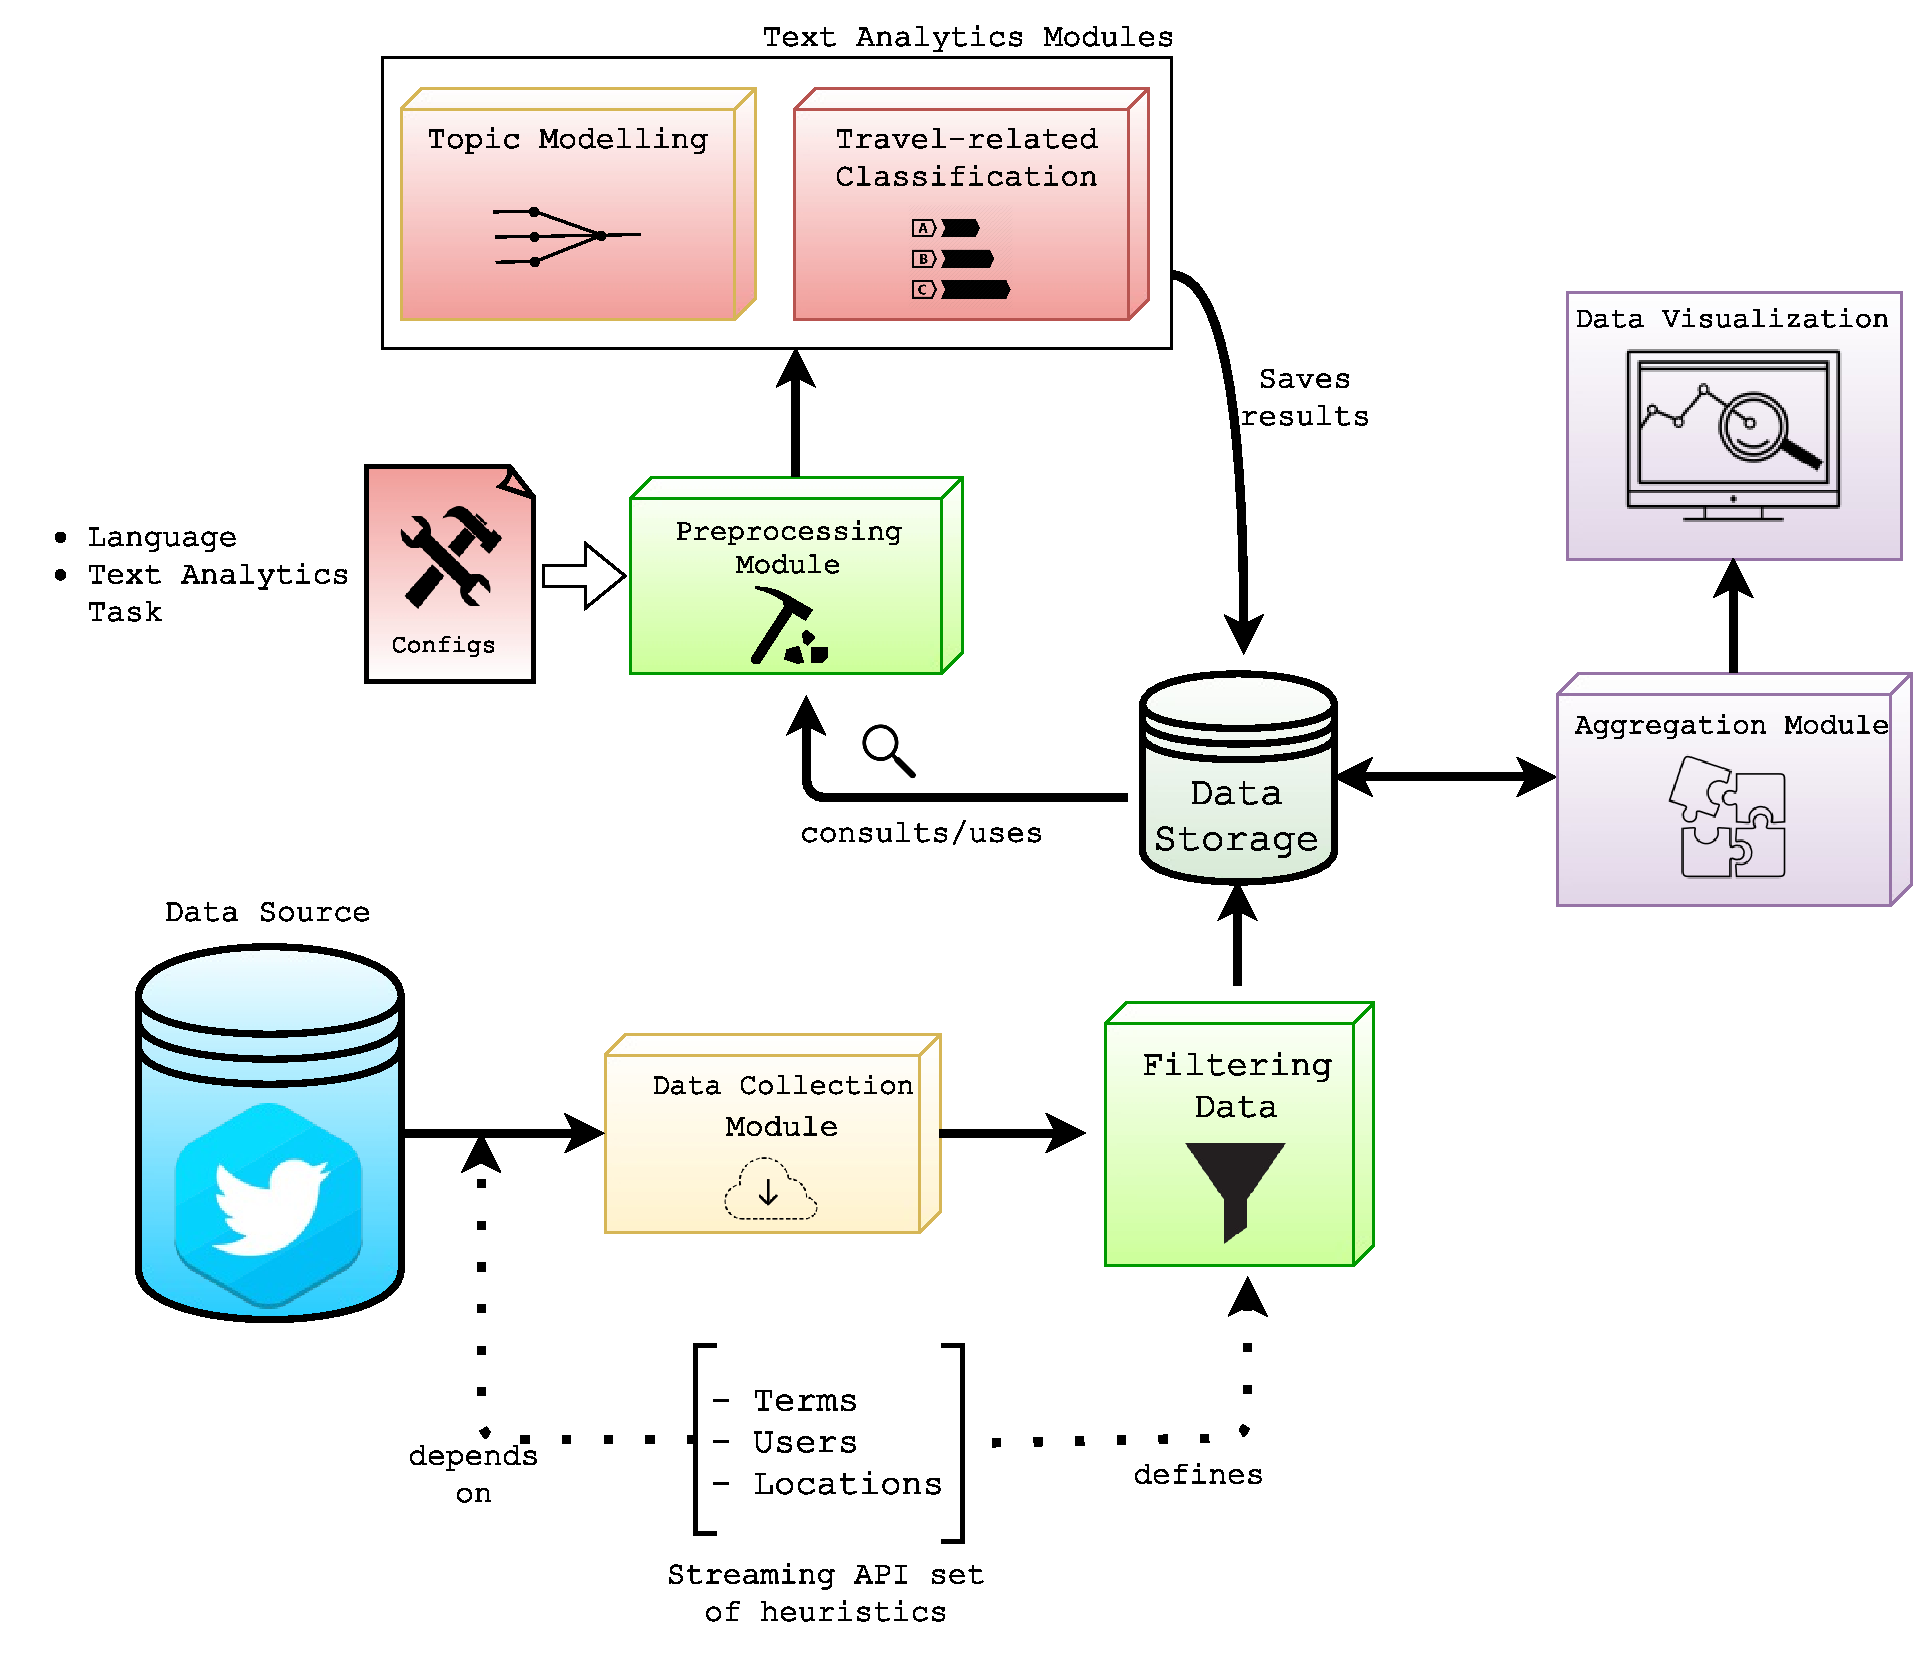
\includegraphics[width=\textwidth]{figures/architecture.pdf}
	\caption[Framework Architecture Overview]{Architecture overview of the proposed framework}
	\label{fig:architecture}
\end{figure}

\section{Data Collection}\label{sec:data_collection}

In Section~\ref{sec:requirements}, we explain the importance of the decision made to the data collection's heuristics. Twitter allows the developers' community two different tools to collect data, the Search and the Streaming APIs. The Search API is based on the RESTful protocol and only looks up for tweets published in the last 7 days, while the Streaming API creates basic endpoints (independent of the REST protocol) and retrieves up to 1\% of the Twitter Firehose~\footnote{Twitter Firehose - is a paid Twitter service that guarantees the delivery of 100\% of the tweets matched with certain criteria.}. Regarding the proposed and developed framework, we chose the Streaming API due to its free-access for the community, smooth integration in the module implementation and due to the availability of real-time information. A positive point about the Streaming API is the three available heuristics to the data collection, allowing the retrieval of tweets that match a specific text query (e.g. tweets with the word \texttt{bus} or \texttt{car}), the retrieval of tweets associated to a variable  number of users - being necessary previous knowledge about these users \textit{ids} - or even the retrieval of tweets located inside a bounding-box~\cite{mac2016effects}. There are two negative points regarding the Twitter Streaming API: first, Twitter imposes limits in its data exploration, where only 400 words can be tracked, 5,000 users can be followed and 25 different bounding-boxes can be explored\footnote{\url{https://dev.twitter.com/streaming/reference/post/statuses/filter} (Accessed on 18/06/2017)}; second, the previously mentioned heuristics cannot be used together, i.e. we can not track specific tweets from an user that match with certain words. Although the negative points, we remain with the choice made, of using the Twitter Streaming API as our source of information and limiting the heuristic to the one that retrieves tweets located inside a bounding-box. Our choice is additionally supported by the need of studying cities and exploring the information derived from it. This way, we know, a priori, that if the data collection method is able to retrieve tweets with precise geo-location then this makes our work easier since the exploration of specific regions of a city is already available taking into consideration the information available in tweets.

After the method selection, as well as the selection of its heuristic, we conduct an experiment regarding the amount of tweets being retrieved by one Twitter client for a city. Twitter has into consideration the number of clients used in the data collection process by tracking the IP address of the machine in the network. This constitutes a restriction to explore several cities with the same client since the Streaming API retrieves only 1\% of the total overcome. In the experiment, we tested the capacity of a client to retrieve all the tweets posted in New York City and used four different clients for it: one defined with the city bounding-box, and the other three defined with bounding-boxes of three boroughs in the city: Bronx, Brooklyn and Manhattan. Considering the bounding-boxes creation, we took support of an open-source \textit{online} tool coined BoundingBox~\footnote{\url{http://boundingbox.klokantech.com/} (Accessed on 23/06/2017)}, which is integrated with the Google Maps API.

Results showed that the client defined with the greatest bounding-box, New York City, was able to retrieve 100\% of the tweets from the three different boroughs. This experiment is consolidated with the work of F. Morstatter et al.~\cite{morstatter2013sample} where it was compared the Streaming API's capacity, regarding geo-located tweets, against the Twitter Firehose. Authors concluded that the percentage of geo-located tweets corresponds to 1-2\% of total overcome from Twitter and the Streaming API is able to retrieve almost 90\% of it. Hence, we do not need to be concerned about how many bounding-boxes are used in the collection process because if we did we would  need to be aware of 90\% of the world, which is not the case.

\section{Data Preprocessing}\label{sec:data_preprocessing}
The extraction of information from text, in particular from social media streams, is an iterative process and requires a segmented and planned pipeline to achieve the final results. In the requirements section (\ref{sec:requirements}), we mentioned some problems of social media streams as the short length and informality of the text message. The informality problem ranges from the writing style of each person to the existence of lots of abbreviations, slang, jargons, \textit{emoticons} and bad usage of punctuation signs. The preprocessing module presented in this section has as main goal the submission of the text messages under several operations in order to remove, or at least, reduce this type of informality characteristics and make easier the work of future tasks.

Below, we enumerate and described the different preprocessing methods implemented:

\begin{itemize}
	\item \textbf{Lower casing:} This operation is responsible for the conversion upper case characters to lower representation. The advantages provided by this operation are centered in the analysis of words written in different ways. An representative example is \texttt{london} and \texttt{London} whose meaning is the same but due to the different case in one letter, its representation/interpretation by text mining techniques may be disparate.
	\item \textbf{Tokenization:} Is the method of dividing each sentence in a list of tokens/words. Since we are dealing with social media content, standard tokenizations techniques available in packages, such as the \texttt{tokenize}~\footnote{\url{http://www.nltk.org/api/nltk.tokenize.html}} of NLTK Toolkit for Python, perform poorly and are not capable of dealing with \textit{\#hashtags}, \textit{@mentions}, abbreviations, strings of punctuation, \textit{emoticons} and unicode glyphs which are very common in Twitter. Having considered this, we used a Twitter-based tokenization package, coined Twokenize and firstly presented by B. O'Connor et al.~\cite{o2010tweetmotif}, which is capable of dealing with these special characteristics of tweets.
	\item \textbf{Punctuation Removal:} Depending on the future task, all signs of punctuation are removed. In this case, every \textit{emoticon} was removed, as well as the symbols \texttt{\#} and {@} which composed the \textit{hashtags} and user mentions.
	\item \textbf{User mentions and \textit{URLs} Removal:} Following the condition of the above mentioned operation, the removal from the text of this type of content depends of the current task.
	\item \textbf{Stop words Removal:} This operation consists in the removing of the most common words in the language in analysis. We used the standard words of the NLTK Corpus package.
\end{itemize}

Regarding other fields in a tweet, this module was also in charge of convert the date of creation of a tweet to the city timezone. The field \textit{created\_at} in a tweet is given in the Coordinated Universal Timezone (UTC) and in order to have knowledge about the most active local hours and days on Twitter, we used the Python timezone package \texttt{pytz} to convert the world timezone to the one desired.

Although the existence of more text preprocessing techniques, in this dissertation we only used the ones previously described since each of them is associated to, at least, one text analytics module whose are described in the following section.

\section{Text Analytics}
The extraction of information from texts can vary in several types depending on the task performed to achieve it. In this dissertation, it was developed different types of analysis having in consideration the text messages.

\subsection{Travel-related Classification}\label{sec:travel_classification}

\emph{Prima facie}, we tried to extract and characterize travel-related tweets from large datasets in order to study the geographical and temporal distributions of such specific content. To be successful in this task we create an automatic text classifier capable of discriminating travel-related tweets from non-related ones. Due to the absence of gold standard datasets in this domain, there was the need of creating a training and testing set of data in order to proceed the experiment and evaluate the performance of the obtained model. Conventional classification tasks in the domain of intelligent transportation systems follow traditional approaches by constructing their group of features using standard bag-of-words techniques. In our experiment, we tried to combine a bag-of-words technique with word embeddings methodologies, producing, for the best of our knowledge, the first travel-related classification model with both type of features.

The word embeddings technique is used by T. Mikolov~et~al.~\cite{mikolov2013efficient} in the implementation of a powerful computational method named \emph{word2vec}. This method is capable of learning distributed representations of words, and each word is represented by a distribution of weights across a fixed number of dimensions. Authors have also proved that such representation is robust when encoding syntactic and semantic similarities in the embedding space.

The training objective of the skip-gram model, as defined by T. Mikolov~et~al.~\cite{mikolov2013linguistic}, is to learn the target word representation, maximizing the prediction of its surrounding words given a predefined context window. For instance, to the word $w_t$, present in a vocabulary, the objective is to maximize the average log probability:

\begin{equation}
\frac{1}{T}  \sum_{t=1}^{T}  \sum_{-c \leq j \leq  c, j \neq 0} \textnormal{log } P(w_{t+j} | w_t)
\end{equation}

where $c$ is the size of the context window, $T$ is the total number of words in the vocabulary and $w_{t+j}$ is a word in the context window of $w_t$. After training, a low dimensionality embedding matrix $\textbf{E}$ encapsulates information about each word in the vocabulary and its use (i.e. the surrounding contexts). For instance, by using the skip-gram model over our datasets we were able to verify that words such as \texttt{ônibus} and \texttt{busão} are used in the similar contexts, as a mode of transport.

Later on, Q. Le and T. Mikolov~\cite{le2014distributed} developed paragraph2vec, an unsupervised learning algorithm operating on pieces of text not necessarily of the same length. The model is similar to \emph{word2vec} but learns distributed representations of sentences, paragraphs or even whole documents instead of words. We used \emph{paragraph2vec} to learn the vector representations of each tweet and tried several configurations in the model hyper-parameterization.

The previous described methods are available in the collection of Python scripts we used in this dissertation, coined \texttt{Gensim}~\footnote{\url{https://radimrehurek.com/gensim/about.html} (Accessed on 20/06/2017)}, presented and lately improved by R. \v{R}eh\r{u}\v{r}ek and P. Sojka~\cite{rehurek2010software}.

The overall experiment regarding the travel-related classification of tweets is described and detailed in Section~\ref{sec:travel_related_classification}. Concluded the experiment, we select the best classifier and used it the implementation of the travel-related module allowing the framework to discriminate potential new tweets related to the transportation domain.

\subsection{Topic Modelling}\label{sec:topic_modelling}

Further developments towards the enrichment of different information provided by the framework took us to the path of topic modelling techniques for text messages. Topic modelling is a text mining technique which goal is the identification of latent topics in a collection of documents. During the last decade, the research community had been using this technique in a vast range of works aiming the test of its applicability in different domains. Here, we also used topic modelling to characterize the different cities and provide this type of information to the framework's end-users.

Latent Dirichlet Allocation (LDA) is a generative statistical model proposed by D. Blei et al.~\cite{blei2003latent} that makes possible the discovering of unknown groups and its similarities over a collection of text documents. The model tries to identify what topics are present in a document by observing all the words that composing it, producing as final result a topic distribution. 

\begin{figure}[htbp]
	\centering
	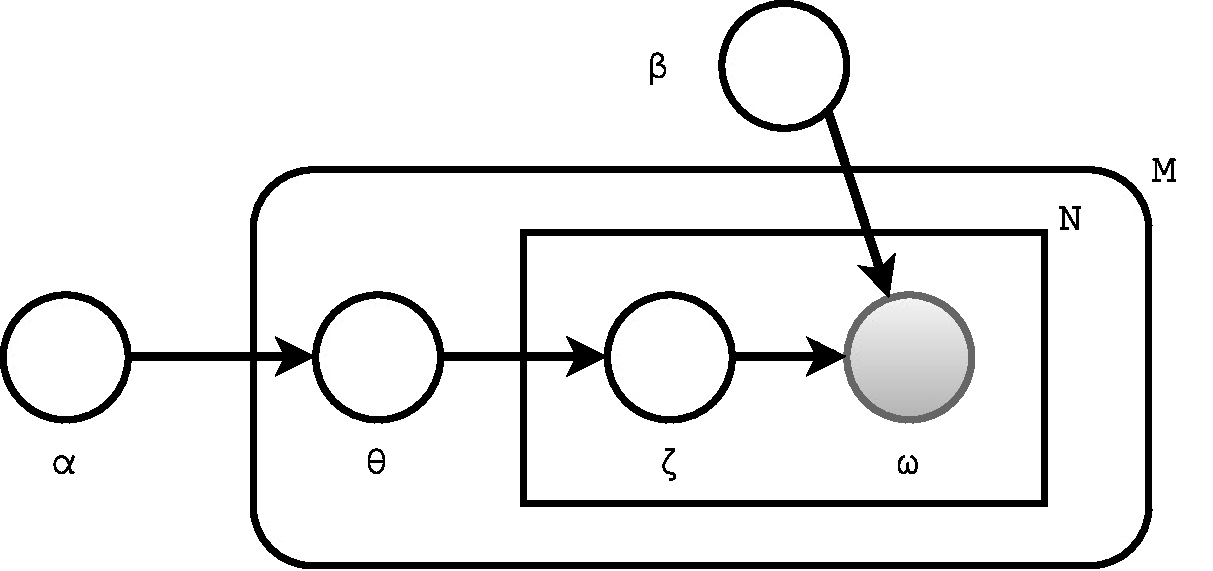
\includegraphics[scale=0.41, keepaspectratio]{figures/lda-model.pdf}
	\caption[Plate notation of LDA by D.Blei et al. ~\cite{blei2003latent}]{Plate Notation of the graphical model representation of Latent Dirichlet Allocation by D.Blei et al. ~\cite{blei2003latent}}
	\label{fig:lda_graphical_model_representation}
\end{figure}

In Figure~\ref{fig:lda_graphical_model_representation} it is illustrated the plate notation to the graphical model of LDA. There, we can observe that for a collection of documents $M$, each one composed by a sequence of $N$ words, the model tries to attribute a per-document topic distribution, using an $\alpha$ dirichlet prior, to a topic-word distribution $\xi$ (associated also with a dirichlet prior $\beta$), inducing that each topic's probability $\theta$ is focused in a small set of words $w$ which characterize that topic.

The most important advantage this model provides is related to the group of features involved in its training process. Conventional application of this model uses only as features a bag-of-words matrix representation~\footnote{Bag-of-words representation matrix is a list of lists, where each entry of the matrix is associated to a sentence of the document and takes the form of a term-frequency vector.}, and for this reason the task of topic modelling becomes very simple since the the frequency of words in the documents are taken into account. Last but not least, LDA model performs two different distributions: (1) distribution of words over topics and (2) distribution of topics over the documents, resulting in the assumption that each document is random mixture of topics, whose in turn are composed by a probabilistic distribution of words.

The cities' characterization provided by our framework centers in the topics being talked about at the time. We conduct an experiment to evaluate if such information could bring added-value for the cities entities and the results although being very promiscuous proved to have potential in certain occasions. The overall experiment is described in Section~\ref{sec:topic_modeling} as well as potential improvements to the generated model.

\subsection{Final Remarks}

The previous mentioned text analytics methodologies were implemented as separate modules in the framework since each of them needs different preprocessing operations over the data. A future interesting improvement to the framework, presented in this dissertation, is the incorporation of an extra module of sentiment analysis that should work together with the two already developed, and provide additional information about the services of a smart city, including the transportation domain.

\section{Data Storage and Aggregation}\label{sec:storage_aggregations}

Besides the few percentage of geo-located tweets provided by Twitter (1-2\% of the total Firehose overcome), this data requires, in the first place, large physical space for storage and, secondly, a tool that allows the easy manipulation and quick access of data. Having considered this, we opted for the use MongoDB, an open-source cross-platform document-oriented database, as the database system for our framework. MongoDB allows the storage of JSON-like documents which is the retrieved format of tweets by the Streaming API. Since in this dissertation we developed the framework as a prototype of a system capable of extracting information related to \textit{smart cities} and transportation services, the large physical space to storage data was not a priority.

MongoDB presents, alongside the high performance, availability and scaling, an inner framework that allows the aggregation of data according to specific user-generated queries. Here, we took advantage of such a pipeline in order to produce interesting statistics regarding the processed data. Map-reduce is the processing paradigm behind the aggregating operations allowing high performance even when applied to large volumes of data, as in this particular case where it is necessary to process thousands or millions of tweets in a short period of time.

\section{Visualization}\label{sec:visualization}

One of the most laborious and time-consuming tasks in the development of this social media based framework was the selection of data visualizations to illustrate the results provided by the previous mentioned modules. Due to the amount of data being processed, the generation of data visualization using an atomic implementation is sometimes poorly in terms of response time. Hence, we needed to adopt a different approach in order to solve this non-efficient procedure.

After a long period of research, we found a solution to this problem by creating a set of routines (bash scripts) that are called periodically (hourly) to execute all type of necessary aggregations and update its corresponding data collections in the database. Then, other routine is invoked to generate all type of data visualizations and store its visual representation in HTML files. In the implementation of this module, these files - containing the data visualization - were embedded inside several view pages. \texttt{Plotly}~\footnote{\url{https://plot.ly/python/}} is a Python graphing library that has available the saving of the visualizations produced in files with HTML format. Besides that, the library offers an extensive range of graphical representations, such as basic charts (bar charts, scatter plots, etc), scientific charts (heatmaps), financial charts (time series) and maps (choropleth, bubble and line maps), which facilitates the construction and designing of dynamic dashboards. Here, we explore mostly the section of basic charts to build simple representations of the results obtained from the analytics phase and also added top lists about some metadata of the tweets, as so the overall, daily and hourly top \textit{hashtags} and uni-grams.

%\section{Summary}
\chapter{Implementação}\label{chap:chap4}

\section*{}

Este capítulo pode ser dedicado à apresentação de detalhes de nível
mais baixo relacionados com o enquadramento e implementação das
soluções preconizadas no capítulo anterior.
Note-se no entanto que detalhes desnecessários à compreensão do
trabalho devem ser remetidos para anexos.

Dependendo do volume, a avaliação do trabalho pode ser incluída neste
capítulo ou pode constituir um capítulo separado.

\section{Secção Exemplo}

%\todofigure{Inserir uma figura sobre o Map/Reduce}

Lorem ipsum dolor sit amet, consectetuer adipiscing elit. Integer
hendrerit commodo ante. Pellentesque nibh libero, aliquam at, faucibus
id, commodo a, velit. 
%\todoline{Escrever sobre o map/reduce}
Duis eleifend sem eget leo. Morbi in est. Suspendisse magna sem,
varius nec, hendrerit non, tincidunt quis, quam. Aenean congue. 
%\todolines{A short entry in the list of todos}{A very long todonote
%  that certainly will fill more than a single line in the list of
%  todos. Just to make sure let's add some more text.} 
Vivamus vel est sit amet sem iaculis posuere. Cras mollis, enim vel
gravida aliquam, libero nunc ullamcorper dui, ullamcorper sodales
lectus nulla sed urna. Morbi aliquet porta risus. 
Proin vestibulum ligula a purus. Maecenas a nulla. 
Maecenas mattis est vitae neque auctor tempus. Etiam nulla dui,
mattis vitae, porttitor sed, aliquet ut, enim. Cras nisl magna,
aliquet et, laoreet at, gravida ac, neque. Sed id est. Nulla dapibus
dolor quis ipsum rhoncus cursus. 

\section{Mais uma Secção}

Lorem ipsum dolor sit amet, consectetuer adipiscing elit. Quisque
purus sapien, interdum ut, vestibulum a, accumsan ullamcorper,
erat. Mauris a magna ut leo porta imperdiet. Donec dui odio, porta in,
pretium non, semper quis, orci. Quisque erat diam, pharetra vel,
laoreet ac, hendrerit vel, enim. Donec tristique luctus risus. Fusce
dolor est, eleifend id, elementum sit amet, varius vitae, neque. Morbi
at augue. Ut sem ligula, auctor vitae, facilisis id, pharetra non,
lectus. Nulla lacus augue, aliquam eget, sollicitudin sed, hendrerit
eu, leo. Suspendisse ac tortor. Mauris at odio. Etiam vehicula. Nam
lacinia purus at nibh. Aliquam fringilla lorem ac justo. Ut nec
enim. 
%\todoref{Citar Map/reduce}

Quisque ullamcorper. Aliquam vel magna. Sed pulvinar dictum
ligula. Sed ultrices dolor ut turpis. Vivamus sagittis orci malesuada
arcu venenatis auctor. Proin vehicula pharetra urna. Aliquam egestas
nunc quis nisl. Donec ullamcorper. Nulla purus. Ut suscipit lacus
vitae dui. Mauris semper. Ut eget sem. Integer orci. Nam vitae dui
eget nisi placerat convallis. 

\begin{lstlisting}[float,language=Java, label=src:mapreduce, caption=Example map and reduce functions for word counting]
map(String key, String value): 
// key: document name 
// value: document contents 
for each word w in value:
EmitIntermediate(w, "1");

reduce(String key, Iterator values):
// key: a word 
// values: a list of counts 
int result = 0;
for each v in values: 
result += ParseInt(v);

Emit(AsString(result))
\end{lstlisting}

Sed id lorem. Proin gravida bibendum lacus. Sed molestie, urna quis
euismod laoreet, diam dolor dictum diam, vitae consectetuer leo ipsum
id ante. Integer eu lectus non mauris pharetra viverra. In feugiat
libero ut massa. Morbi cursus, lorem sollicitudin blandit semper,
felis magna pellentesque lacus, ut rhoncus leo neque at tellus. Sed
mattis, diam eget eleifend tincidunt, ligula eros tincidunt diam,
vitae auctor turpis est vel nunc. In eu magna. Donec dolor metus,
egestas sit amet, ultrices in, faucibus sed, lectus. Etiam est enim,
vehicula pharetra, porta non, viverra vel, nunc. Ut non sem. Etiam nec
neque. 

\section{Resumo ou Conclusões}

Proin vehicula pharetra urna. Aliquam egestas
nunc quis nisl. Donec ullamcorper. Nulla purus. Ut suscipit lacus
vitae dui. Mauris semper. Ut eget sem. Integer orci. Nam vitae dui
eget nisi placerat convallis. 

\chapter{Conclusões e Trabalho Futuro} \label{chap:concl}

\section*{}

Deve ser apresentado um resumo do trabalho realizado e apreciada a
satisfação dos objetivos do trabalho, uma lista de contribuições
principais do trabalho e as direções para trabalho futuro.

A escrita deste capítulo deve ser orientada para a total compreensão
do trabalho, tendo em atenção que, depois de ler o Resumo e a
Introdução, a maioria dos leitores passará à leitura deste capítulo de
conclusões e recomendações para trabalho futuro.

\section{Conclusão}

\subsection{Possíveis Vantagens e Desvantagens}

\section{Trabalho Futuro}

\subsection{Planeamento do Desenvolvimento}

\vspace*{12mm} 
 

%%----------------------------------------
%% Final materials
%%----------------------------------------

%% Bibliography
%% Comment the next command if BibTeX file not used, 
%% Assumes that bibliography is in ``myrefs.bib''
\PrintBib{myrefs}

%% Comment next 2 commands if numbered appendices are not used
\appendix
\chapter{Loren Ipsum} \label{ap1:loren}

Depois das conclusões e antes das referências bibliográficas,
apresenta-se neste anexo numerado o texto usado para preencher a
dissertação.

\section{O que é o \emph{Loren Ipsum}?}

\emph{\textbf{Lorem Ipsum}} is simply dummy text of the printing and
typesetting industry. Lorem Ipsum has been the industry's standard
dummy text ever since the 1500s, when an unknown printer took a galley
of type and scrambled it to make a type specimen book. It has survived
not only five centuries, but also the leap into electronic
typesetting, remaining essentially unchanged. It was popularised in
the 1960s with the release of Letraset sheets containing Lorem Ipsum
passages, and more recently with desktop publishing software like
Aldus PageMaker including versions of Lorem Ipsum~\citep{kn:Lip08}. 

\section{De onde Vem o Loren?}

Contrary to popular belief, Lorem Ipsum is not simply random text. It
has roots in a piece of classical Latin literature from 45 BC, making
it over 2000 years old. Richard McClintock, a Latin professor at
Hampden-Sydney College in Virginia, looked up one of the more obscure
Latin words, consectetur, from a Lorem Ipsum passage, and going
through the cites of the word in classical literature, discovered the
undoubtable source. Lorem Ipsum comes from sections 1.10.32 and
1.10.33 of ``de Finibus Bonorum et Malorum'' (The Extremes of Good and
Evil) by Cicero, written in 45 BC. This book is a treatise on the
theory of ethics, very popular during the Renaissance. The first line
of Lorem Ipsum, ``Lorem ipsum dolor sit amet\ldots'', comes from a line in
section 1.10.32.

The standard chunk of Lorem Ipsum used since the 1500s is reproduced
below for those interested. Sections 1.10.32 and 1.10.33 from ``de
Finibus Bonorum et Malorum'' by Cicero are also reproduced in their
exact original form, accompanied by English versions from the 1914
translation by H. Rackham.

\section{Porque se usa o Loren?}

It is a long established fact that a reader will be distracted by the
readable content of a page when looking at its layout. The point of
using Lorem Ipsum is that it has a more-or-less normal distribution of
letters, as opposed to using ``Content here, content here'', making it
look like readable English. Many desktop publishing packages and web
page editors now use Lorem Ipsum as their default model text, and a
search for ``lorem ipsum'' will uncover many web sites still in their
infancy. Various versions have evolved over the years, sometimes by
accident, sometimes on purpose (injected humour and the like). 

\section{Onde se Podem Encontrar Exemplos?}

There are many variations of passages of Lorem Ipsum available, but
the majority have suffered alteration in some form, by injected
humour, or randomised words which don't look even slightly
believable. If you are going to use a passage of Lorem Ipsum, you need
to be sure there isn't anything embarrassing hidden in the middle of
text. All the Lorem Ipsum generators on the Internet tend to repeat
predefined chunks as necessary, making this the first true generator
on the Internet. It uses a dictionary of over 200 Latin words,
combined with a handful of model sentence structures, to generate
Lorem Ipsum which looks reasonable. The generated Lorem Ipsum is
therefore always free from repetition, injected humour, or
non-characteristic words etc. 


%% Index
%% Uncomment next command if index is required, 
%% don't forget to run ``makeindex mieic'' command
%\PrintIndex

\end{document}
